%
%
\documentclass{report}
% PAGE DIMENSIONS
\usepackage{geometry}
\geometry{a4paper,margin=3.5cm}

% PACKAGES
\usepackage{graphicx} %support the \includegraphics command and options
\usepackage{fancyhdr} % Headers/footers (should be set AFTER setting up the page geometry and before hyperref)
\usepackage{color}
\usepackage{eso-pic} %background pictures
\usepackage[latin1]{inputenc}
%\usepackage[danish]{babel}
%\usepackage[T1]{fontenc}
%\usepackage{courier}
\usepackage{csquotes}
\usepackage{booktabs} % for much better looking tables
\usepackage{tabularx}
\usepackage{slashbox}
\usepackage{array} % for better arrays (eg matrices) in maths
\usepackage{paralist} % very flexible & customisable lists (eg. enumerate/itemize, etc.)
\usepackage{verbatim} % adds environment for commenting out blocks of text & for better verbatim
\usepackage{alltt} %improved verbatim
\usepackage{titlesec} %to modify \chapter, \section, etc appearance
\usepackage{hyperref} %til links, email etc - giver ogs bookmarks i pdf filen
%\usepackage{dirtree} %directory trees
\usepackage{subfig} %make it possible to include more than one captioned figure/table in a single float
\usepackage{float} %float positioning etc
\usepackage{amsmath,amsfonts,amssymb,amsthm} %AMS' packages for symbols, theorems etc.
\usepackage{xfrac} %for nicefrac{}{}
\usepackage{wrapfig}
\usepackage{multicol}
\usepackage{footnote}
\usepackage{perpage}
\usepackage{ctable}
\usepackage[intoc]{nomencl} %for abbreviations list
\usepackage{listings} %for source code listings
\usepackage{marginnote} %Margin notes - use \marginnote{}
%\usepackage[textsize=footnotesize]{todonotes} %the ''disable'' option removes notes
\usepackage{url}
\usepackage{multirow}
\usepackage[normalem]{ulem} %underline, and variations thereof
%\usepackage[parfill]{parskip} %Activate to begin paragraphs with an empty line rather than an indent

% Bibliography appearance
\usepackage[style=numeric,natbib=true,sortcites=true,block=space,backend=bibtex8]{biblatex}
\bibliography{content/bibliography}

% marginnote package options
\renewcommand*{\marginfont}{\color{red}\sffamily} %red, sans-serif
\reversemarginpar %margin notes on left side

% makes footnotes in tables possible (perpage package)
\MakePerPage{footnote}
\makesavenoteenv{tabular}

% listings package settings
\lstloadlanguages{Matlab,[ANSI]C++,[Visual]C++}
\lstset{
  basicstyle=\ttfamily\small,
  %aboveskip=12pt,
  %belowskip=12pt,
  %frame=l,
  numbers=left,
  numberstyle=\ttfamily\tiny,
  numbersep=8pt,
  captionpos=b,
  tabsize=4,
  extendedchars=true,
  breaklines=true,
  showspaces=false,
  showtabs=false,
  keywordstyle=\color{blue},
  escapeinside={(*�}{�*)},
  %rangeprefix=,
  %rangesuffix=,
  includerangemarker=false,
  %stringstyle=\color{white}\ttfamily,
  %commentstyle=\color{white} %''cheat'' to hide comments
  xleftmargin=10pt,
  %backgroundcolor=\color{lightgray},
  showstringspaces=false,
  morekeywords={step,impulse,pzmap,bode,freqz}
}
%\renewcommand*\lstlistingname{Code}

% hyperref package settings
\hypersetup{
    unicode=true,          % non-Latin characters in Acrobat�s bookmarks
    pdftoolbar=true,        % show Acrobat�s toolbar?
    pdfmenubar=true,        % show Acrobat�s menu?
    pdffitwindow=false,     % window fit to page when opened
    pdfstartview={FitH},    % fit page to the window Horizontal/Vertical
    pdftitle={TITLE},    % title
    pdfauthor={Alexander Adelholm Brandbyge, Frederik Hagelskj�r, Rudi Hansen, Leon Bonde Larsen, Kent Stark Olsen, Kim Lindberg Schwaner},% author
    pdfsubject={SUBJECT},   % subject of the document
    pdfkeywords={DTMF} {keyword2} {SDU}, % list of keywords
    pdfnewwindow=true,      % links in new window
    colorlinks=false,       % false: boxed links; true: colored links
    linkcolor=red,          % color of internal links
    citecolor=green,        % color of links to bibliography
    filecolor=magenta,      % color of file links
    urlcolor=cyan,           % color of external links
    plainpages=false
}

% Headers and footers
\pagestyle{fancy} % options: empty , plain , fancy
\setlength{\headheight}{15pt}
%\lhead{\nouppercase{\rightmark}}
\lhead{\nouppercase{\leftmark}}
\chead{}
%\rhead{}
\rhead{\nouppercase{\rightmark}}
\lfoot{}
\cfoot{}
\rfoot{\thepage}

\fancypagestyle{plain}{% Using the plain-style to be able number pages, but with an empty header! (using the report document class makes this nearly obsolete)
 \fancyhf{}
 \renewcommand{\headrulewidth}{0pt}
 \fancyfoot[RO]{\thepage}
}

%%% Contents appearance
\usepackage[]{tocbibind} % Put the bibliography in the ToC (Opts: nottoc,notlof,notlot)
\setcounter{tocdepth}{3} % set how many levels the table of contents displays. default=3
\usepackage[titles,subfigure]{tocloft} % Alter the style of the Table of Contents

% \includegraphics default folder
\graphicspath{{content/graphics/}}

% Number by section
%\numberwithin{equation}{section}
%\numberwithin{figure}{section}
%\numberwithin{table}{section}

% Paragraphs (handled by the parskip package currently?)
%\setlength{\parindent}{0pt}
%\setlength{\parskip}{2ex plus 0.5ex minus 0.2ex}

% Float positioning control
\setcounter{topnumber}{2}
\setcounter{bottomnumber}{2}
\setcounter{totalnumber}{3}
\renewcommand{\topfraction}{0.85}
\renewcommand{\bottomfraction}{0.85}
\renewcommand{\textfraction}{0.15}
\renewcommand{\floatpagefraction}{0.4}

% Header colour
\definecolor{FrontpageHeadingColor}{RGB}{5,5,60}%Heading colour definition

% Chapter name formatting
\titleformat
  {\chapter}%command
  [display]%shape
  {\normalfont\huge\bfseries}%format
  {\normalfont\Large\scshape\chaptertitlename\ \huge\thechapter}%label
  {10pt}%sep
  {\Huge}%before

% make nomenclature and change its heading/toc text (see nomencl package)
\makenomenclature
\renewcommand{\nomname}{Abbreviations}
%
%  * Pass this line to MakeIndex:
%    %bm.nlo -s nomencl.ist -o %bm.nls
%
%  * Use \nomenclature{abbr}{discriptive text} to add an entry to the 
%    abbreviations list (best done where the abbreviation first occurs in the text)
%  * Example:
%    \nomenclature{ADHD}{Attention Deficit Hyperactivity Disorder}

\begin{document}
%
% Front page
\pagenumbering{alph} %frontpage numbered with a letter
\begin{titlepage}%
\currentpdfbookmark{Front page}{front_page}%hyperref pdf bookmark
\AddToShipoutPictureBG*{%background picture	
 \put(0,0){
  \parbox[b][\paperheight][b]{\paperwidth}{%\parbox[position][height][inner-pos]{width}{text}
   \vfill
   %\begin{flushright}
   
\includegraphics[width=0.43\paperwidth,trim=110 0 0 0]{sdu_seal.pdf}%trim=l b r t
   %\end{flushright}
   \vspace*{2.9cm}
  }
 }
}
\begin{flushright}

\includegraphics[scale=0.73]{sdu_logo.pdf}
\end{flushright}
\vspace*{2.7cm}
%
%\textsf{\Large{\textbf{Gruppe 1}}}
%
%\vspace*{0.3cm}
\setlength{\extrarowheight}{1.5pt}
\begin{tabular}{@{}l l}
	\textsf{\large{311289}} & \textsf{\large{Alexander Adelholm Brandbyge}}\\
	\textsf{\large{251289}} & \textsf{\large{Frederik Hagelskj�r}}\\
	\textsf{\large{260387}} & \textsf{\large{Rudi Hansen}}\\
	\textsf{\large{150179}} & \textsf{\large{Leon Bonde Larsen}}\\
	\textsf{\large{040282}} & \textsf{\large{Kent Stark Olsen}}\\
	\textsf{\large{160788}} & \textsf{\large{Kim Lindberg Schwaner}}
\end{tabular}
\setlength{\extrarowheight}{0pt}
\vspace*{1.5cm}
\\
\textsf{\Huge{\textbf{\textcolor{FrontpageHeadingColor}{A generic protocol stack}}}}
\vspace*{0.5cm}
\\
\textsf{\Large{\textbf{\textcolor{FrontpageHeadingColor}{DTMF as information carrier}}}}
\vfill
\textsf{\\Faculty of Engineering\\
University of Southern Denmark\\
Niels Bohrs All� 1\\
5230 Odense M\\
Denmark}
\vspace*{10pt}
\\
\textsf{www.sdu.dk/tek\\
+45 6550 7303\\
tek@tek.sdu.dk}
\end{titlepage}%
%
% Abstract (un-numbered chapter)
\pagenumbering{roman} %until main content we use roman page numbering
\chapter*{Abstract}\addcontentsline{toc}{chapter}{Abstract}
This project is based on the given assignment to create a protocol stack which
use DTMF tones as information carriers, furthermore this has to be done through air
by speaker and microphone. The team agreed on pursuing a secondary objective which
was to develop an application programming interface for easy-to-use utilisation of
the protocol stack.

It is natural therefore to use the layers described in the OSI-model to define
the implementation of the protocol stack itself, and for the composition of the report.
Interdisciplinarity is a big concern for this project as networking- and datacommunication
theory is mixed with the basics of, digital signal processing, software development,
and C++ programming skills. Thus, this report will reflect these skills used to analyse given
problem statements and solving them.

Everything points in the direction of accomplishment of the objective as a fairly stable 
protocol stack was implemented, though it is not efficient compared to state of the art
data communication systems which exist today. In time of writing, the application programming
interface is still under development.

The result work as a proof of concept, that DTMF tones can be used as information carriers
when the data is transported in air. The significance of creating this proof have given a
great insight in topics regarding the basics of, networking and data communication,
digital signal processing, software development, and C++ programming.
%
% Preface (un-numbered chapter)
\chapter*{Preface}\addcontentsline{toc}{chapter}{Preface}
Wee

%
% Table of contents, figures, tables, listings and abbreviations
\clearpage
\tableofcontents
\listoffigures
\listoftables
\lstlistoflistings\addcontentsline{toc}{chapter}{Listings}
\printnomenclature
%
%
% MAIN CONTENT
\clearpage
\pagenumbering{arabic} %''normal'' arabic numbering from here on out
%
%
\chapter{Introduction}
This is an introduction. Is should contain things like..

This project is devised as a part of the B.Sc. Robot Systems Engineering, 3rd term course at the Faculty of Engineering, University of Southern Denmark, Odense autumn 2011. The implicit goal is to obtain knowledge of computer applications for signal handling. The weight will mainly lay at understanding analogue and digital signals, and integrate this handling in computer applications where computer architecture, operating systems, and data communication will enter into as significant competences.

As the DSMI\footnote{The Engineering Education Model of the University of Southern Denmark} model is used as a framework for this particular education, it is required for the students participating in this course to formulate a strategy for solving a assignment in teams.
\section{Requirements}
This project has in many ways an experimental approach, where it is largely up to the students to figure out how to solve this assignment. This is duo to the requirement of building a protocol stack which uses DTMF tones as data carriers. The exact requirements of the assignment are listed below:

\begin{itemize}
\item Computers have to communicate by exchanging sound.
\item DTMF tones have to be used and a protocol stack have to be build.
\item Information have to be exchanged between computers.
\item A distributed application have to be developed in C++.
\item The architecture have to be layered.
\item It is required that the application perform some meaningful task.
\end{itemize}
\section{Report structure}
The report will be split into several chapters which each explain the different areas that have been explored to fulfil the requirements of this assignment. In chapter \ref{chap:general} the general concepts will be discussed. Chapter \ref{chap:physical} will delve at the physical layer, which define the rules of the data transmission itself and how it should handle this data regarding the upper layer. Chapter \ref{chap:dll} will contain an overview of the data link layer, which explains concepts around the frame, flow control, and error control. Chapter \ref{chap:transport} will explain the workings behind the process-to-process communication. The backbone which control the flow of data between layers is explained in chapter \ref{chap:backbone}. Utilisation and concepts of the application programming interface which acts as the easy-to-use feature of the protocol stack is explained in chapter \ref{chap:api}. Chapter \ref{chap:test} will explain about the test tool that have developed to test each layer separately for stability issues. Experiments conducted will be held in chapter \ref{chap:experiments}. A discussion of the process, solutions, and the results takes place in chapter \ref{chap:discussion}. The conclusion will reside in chapter \ref{chap:conclusion}.

Along with this report a CD will be attached, which contain all material produced during this process. The source and the distributed application will be included on the CD as well.
\section{Project members}
This section will serve as an introduction to each of the project group members. It briefly tells which parts of the project, each member has concerned himself with mostly and what role he has been filling. These roles originate from the Belbin team role model. As the project was begun, the group sat down and discussed which roles they would like to try and fill. They were selected out of a wish to learn what a particular role would involve, and not necessarily what each member is best at.

\begin{description}
\item[Alexander] Has primarily been working on the general architecture of the project, and the developement of the backbone class + associated buffers.
\item[Frederik] Was primeraly responsible for testing. Working with the development of a uniform test-program for debugging and performance testing.
\item[Kent]
has been working with the physical layer which is the lowermost layer of the OSI-model. It has demanded for his skills in terms of understanding the basics of, networking and data communication, digital signal processing, software development, and C++ programming. As a team player Kent is still challenged and he still needs to work on handling conflicts with greater dexterity.
\item[Kim] is a slem bandit
\item[Leon] is a slem bandit
\item[Rudi] is a slem bandit
\end{description}
%
\chapter{General concepts}
Introduction..
\begin{itemize}
 \item An overview.
 \item About network layers, OSI model, what does it mean and why split it in to parts like that?
 \item Explain DTMF - what are those?
 \item Naming conventions? Such as, our library is the ''Dtmf library''
\end{itemize}
%
\chapter{Design decisions}
%available alternatives, decisions made, theory of operation
%\begin{itemize}
%\item ''our'' layers	
%\item backbone
%\item test class
%\item application to use with our network
%\end{itemize}

To facilitate development, the sound sound network protocol is divided into layers corresponding to those of the OSI model. The functionality of each layer and it's responsibilities will, at first, be descriped seperately in this chapter. yada yada
\section{Data link layer} %Overview and considerations concerning -

\begin{figure}[htb]%%PDF figure if possible
	\begin{center}
	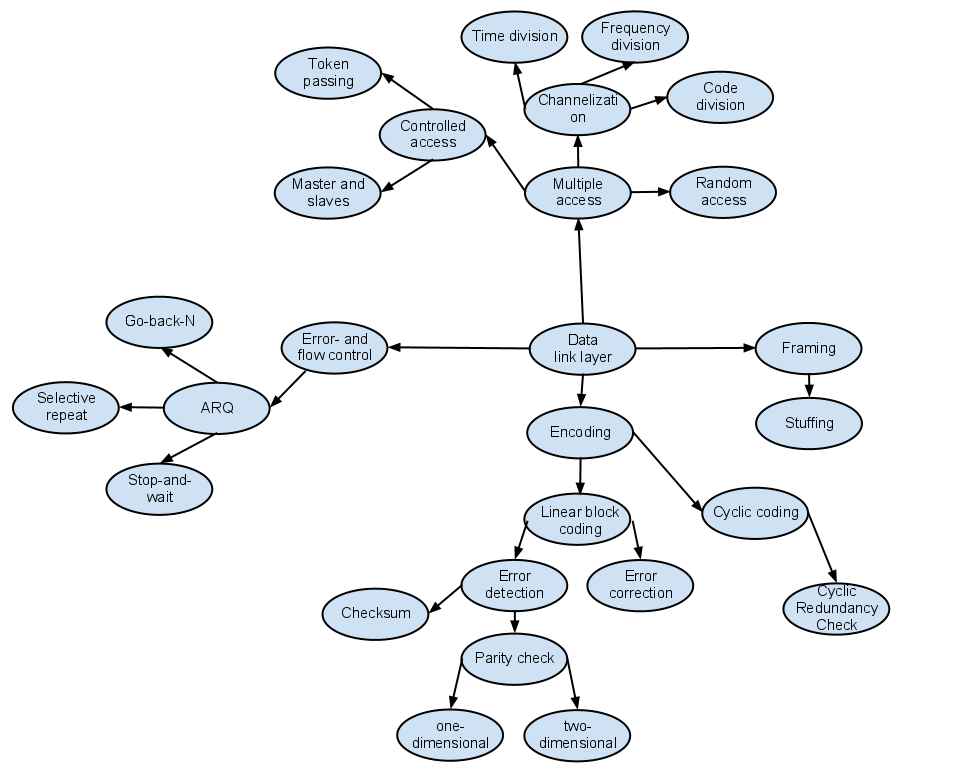
\includegraphics[scale=0.4,trim=0 0 0 0]{dll_bobler.png}%trim=l b r t
	\caption{Things to consider concerning data link layer}
	\label{fig:dll_bobler}
	\end{center}
\end{figure}

\subsection{Encoding}
First thing to consider is the encoding of signals. Since there are sixteen
different DTMF combinations, each tone can carry four bits.

The only type of error to consider is the situation where a tone is
misinterpreted, which leads to a four bit burst error. Therefore the system
should be designed specifically to detect errors of this type. Since the media
is considered to be very noisy, transmissions should also be kept as short as
possible.

A two dimensional parity check will be able to detect burst errors of the
proposed size, so this is the choice. Implementing the parity check as a
four-by-four matrix will make it possible to transfer two bytes with a frame of
three bytes.

Example: We want to transmit the two bytes 0011 0101 and 0101 1110. The data
link layer puts these in a four by four matrix and calculates the parity bits by
adding the rows and columns:

\begin{table}[htb]
	\begin{center}
	\begin{tabular}{c|c}
	0011 & 0 \\
	0101 & 0 \\
	0101 & 0 \\
	1110 & 1 \\
	\hline
	1101 & \\
	\end{tabular}
	\end{center}
	\caption{Two-dimensional parity check}
	\label{tab:two_dimensional_parity_check}
\end{table}

Instead of as normally done to increase the size of each row by one to contain
the parity bit, the parity bits are transmitted together as a redundant byte. In
the case of this example the transmission would be:

\begin{table}[htb]
	\begin{center}
	\begin{tabular}{c|c|c|c|c|c}
	0011 & 0101 & 0101 & 1110 & 0001 & 1101 \\
	\end{tabular}
	\end{center}
	\caption{Bytes to be transmitted}
	\label{tab:bytes_to_be_transmitted}
\end{table}

Each four bit nipple is now transmitted an a DTMF-tone. Should one of the tones
be misinterpreted, the receiving data link layer would get a mismatch of the
parity bits for example:

\begin{table}[htb]
	\begin{center}
	\begin{tabular}{c|c}
	0011 & 0 \\
	0101 & 0 \\
	0000 & 0 \\
	1110 & 1 \\
	\hline
	1000 & \\
	\end{tabular}
	\end{center}
	\caption{Failed parity check}
	\label{tab:failed_parity_check}
\end{table}

This will lead to the frame being discarded. Though in some cases it will be
possible to correct the error and find the original nibble, this is not
recommended, since more than one tone might be corrupted. Errors in the
redundant byte will also lead to the discarding of the transmission.

\subsection{Flow control}
The next thing to consider is flow control. Since the DTMF-system
cannot be used as full-duplex, piggybacking is impossible. This means that at
some point the receiver must reply. This reply will also be of six-tones, and
therefore it might as well contain information about witch frames to resend. In
other words a selective repeat system is preferred

To introduce a selective repeat system, additional redundancy is needed.

By using three bits for the sequence number, redundancy is kept as low as
possible while still benefiting from pipelining. The sender transmits eight
frames (fourty eight tones) and then waits for the receiver to reply with one
frame (six tones).

\subsection{Framing}
It is presumed that the physical layer will provide a starting point for each
transmission. If this is not the case,
additional flags will be needed in between the frames, again leading to the need
of stuffing.

Next thing to consider is multipoint. There are three options: A token
network, a time division network or a code division network. Time division
requires a level of timing the interface layer is unable to deliver.
Code division leads to the need for larger frames or if implemented with the
proposed frame size, a lot of unused frames in a small network. This leaves us
with a token passing network, so this is the choice.

Three bits will control the addressing, all identifying the receiver, since info
about sender is not needed at this level. Thereby the protocol allows networks
of up to eight stations.

The selective repeat system and the token network introduces the need for different frame types.
The type field will consist of two bits, at the same time controlling
the token and indicating frame types. Rules must be implemented to keep the token circulating.

\begin{table}[htb]
	\begin{center}
	\begin{tabular}{|c|ll|}
		\hline
		00 & Has no token & Reply from receiver \\
		\hline
		01 & Has no token & Passes token to addressed station \\
		\hline
		10 & Has token & Accepts token from addressed station \\
		\hline
		11 & Has token & Data frame for addressed station \\
		\hline
	\end{tabular}
	\end{center}
	\caption{Protocol for type field}
	\label{tab:protocol_for_type_field}
\end{table}

Reply frames has type 00 and sequence number 111 (to prevent legal 0:0:0
frames). Each bit of the data byte corresponds to a sequence number and has
value 1 for accepted and 0 for resend.

Token passing is controlled by the backbone architecture of the system and is
implemented in the data link layer. When the token is offered,
there is a window of response time, wherein the station must reply by accepting
the token. If there are no reply during the window, the token is offered to the
next station. 

The backbone has a routine for asking the data link layer whether
it has the token or not. If there are data to send, this is initialized by the
backbone, else the token is passed to the next station. These functionalities
are implemented as public methods in the data link layer.

This leads to the following format of a frame: 

\begin{table}[htb]
	\begin{center}
	\begin{tabular}{|ccc|c|c|}
		\hline
		type (2 bits) & address (3 bits) & sequence (3 bits) & data (8 bits) & parity
		(8 bits)  \\
		\hline
	\end{tabular}
	\end{center}
	\caption{Final frame format}
	\label{tab:final_frame_format}
\end{table}
\section{Transport layer}
In the OSI model, the session and transport layers handle process-to-process sessions (chiefly used when a more permanent connection is required for synchronous transfer, for example) and communication, respectively. When initially exploring ideas for this networking protocol, one wish was that it should be able to serve more than just one application at a time. This brings a need for such process-to-process delivery that the transport layer protocols provide.

\subsection{Addressing processes}
The data link layer in our model takes care of the node-to-node delivery, where each node has an address. This address is, however, not at all useful \textit{after} a node's data link layer has received data and passed it on to the transport layer. Thus, we need a different addressing method: A port number.\footnote{Port number, in this text, is separate from the port number associated with a process by it \textit{binding} via some kind of Internet socket. Still, the term is used, as it's purpose is identical to the ''normal'' port number.}

The port number assigned to a certain server\marginnote{Define server and client as used here} application must be known to the client before it sends anything. That is the only way the . Here, we select the port number to be eight bits long. This reasoning behind this choice is, that we will not at all be able to serve more than a couple of applications at a time, at the most. Add to that, that we wish to keep a minimal overhead size (a higher port number would add more bits to the header), as we don't have a lot of bandwidth to begin with.

\subsection{Datagram}

Much like UDP

\nomenclature{UDP}{User datagram protocol}
\nomenclature{TCP}{Transmission control protocol}

\subsection{Placeholder}
From the application, the transport layer expects to just receive a stream of bytes. The order in which the bytes are received is significant, but the data they contain is not.

%\subsection{Segmentation?}

\begin{table}[htb]
 \centering
 \begin{tabular}{c}
  
 \end{tabular}
 \caption{Datagram format}
 \label{tab:Datagram_format}
\end{table}
%%%%%%%%%%%%%%%%%%%%%%%%%%%%%%%%%%%%%%%%%%%%%%%%%%%%%%%%%%%%%%%%%%%%%%%%%%%%%%%%
% IN:
% ----
% * Byte-array
% * Source port number       \
% * Destination port number   \_ (or do we know this already?)
%
% OUT:
% ----
% HEADER                        DATA
% 

% ''session''-delen er lidt ude i kulden? connection oriented transport layer protokol kan det, vi gerne vil?

% sekvensering
% process-process
% process ID (PID) / ''port'' number
% (de)-multiplexing
% in/out queue-buffer (one for each port)
%   overflow
%   unreachable/queue non-existant
% reserved ports for system messages?
% flow control, we don't need (?)
% unrealiable sending ?
% connectionless service ?
% congestion, we dont care?


% socket address = ''data link layer''-address + port number


%\section*{Transport and session layers}
%This layer opens and manages the connection and routes between different
%processes on the station. It is also responsible for segmentation and reassembly
%of packages.
%
\chapter{Implementation}
How was it made?

\begin{itemize}
\item each layer
\item backbone
\item test class
\item application to use with our network
\end{itemize}
%
\chapter{Experiments}\label{chap:experiments}
Throughout development a lot of testing have been done towards debugging the program. However this chapter is only concerned about tests of the systems conditions. Tests beformed to get a knowlegde of the layers abilities concerning performance and reliability. Thus it will be possible to gain an overwiev of the application. The results of souch tests will ofcourse depend the used computers ability, standard laptops were used. 


This chapter descripes the perfomed tests and the results gained.






%
\chapter{Discussion}\label{chap:discussion}
The main idea about implementing the generic protocol stack has been to find an approach
where each member of the team was able to dig deeply into the essence of the
professions while still making it easy to compile the different parts of the
project into a coherent solution.

The chosen approach was to define clean interfaces between the software layers
in the form of predefined buffers. This has proven to be a powerful tool, since
each layer has been debugged and tested individually. Also a lot of potential
problems about the overall flow- and software control was avoided, since all
methods and loops were connected in the backbone program.

The architecture has provided a certainty of maximum reuse of
code and have efficiently avoided unnecessary coupling in the software. Because
of the bold ambition to create a compiled library for other developers to use, the problem reached a
size, where efficient programming was imperative. Time was also an issue and
again the procedure has proven most beneficial because each team member has been
able to work and test independent of the others, thereby avoiding time wasted in
waiting for other parts to finish.

The respective layers have been developed using an iterative approach, where
the individual team member has worked on his part and then presented it to the rest
of the group either by internal documentation on the project wiki, input to the
report, demonstration programs or by giving short lectures in the subject. This
way the team has been able to work efficiently while still pulling together.

The distribution of team roles has been a challenge, mostly because it implies a
new way of thinking in behaviour and responsibilities instead of duties and
fields of expertise. It was an informed choice to select the team roles from a
point of learning and not a point of experience. This decision ensured that
all members started on equal feet, but also imbued some difficulties of breaking
old patterns. It has provided some serenity to the work, knowing that one does
not have to be mindful of the entire project, trusting that other team members
will do their part.

Professionally the project has given hands on experience of the OSI layers
taught in data communication and a much greater understanding of the material.
Developing a large software system leads to considering the UML language and
advantages of object oriented programming, supporting the lectures in software
development. Since all members of the team have contributed to the source code,
a much greater experience in C++ programming has been obtained. Finally the
analysis of the problem and to some extend implementing the tone detection
system has lead to a greater understanding of digital signal processing.
\chapter{Conclusion}\label{chap:conclusion}
Questions to be answered:

To what extend was it possible to make an API that implements a DTMF based
network?
How did the system perform during test? 
Are there things that should be testet further?

To what extend does the physical layer work? 
The physical layer works like a charm, according to table \ref{tab:exp_phys_speaker} a bit rate around $110\sfrac{bit}{s}$ can be reached without compromising the reliability too much. Several optimisation possibilities are available, but not needed as stability is not an issue.

  To what extend does the data link layer work? 
The data link layer is able to process a packet and enclose it in a sequence of
frames to be sent. It is also able to receive frames and to process them into at
packet to be delivered to the transport layer. The data link layer is also able
to control a token based network in a way that allows collision free half duplex
communication. 

  How did the data link layer perform during test? The data link
layer performed well under test and handles communication with up to sixty
percent errors, though this amount of errors makes it very slow. With more than
sixty percent errors all time goes into contol talk and almost no frames are
transmitted.

  What could make it even better?
If it is possible to find a way of using a sliding window instead of the eight
byte list currently implemented. There is currently a lot of transmission time
being wasted in sending lists shorter than eight entries. Other changes could be
considered to handle cases where a crucial frame is lost. For example the case
where a reply is lost which results in some waiting time and the entire list
being resend.

To what extend does the transport layer work? 
How did the transport layer perform during test?
What could make it even better?

To what extend does the API layer work? 
How did the API layer perform during test?
What could make it even better?

To what extend does the Backbone work? 
The backbone class works as expected. It is able to dispatch work to the correct layer objects, based on the state of the internal buffers and layers.
How did the backbone perform during test?
The backbone has not been tested, as it is meaningless to test it without the actual layers combined. Since the final assembly has not been completed at the time of writing, any backbone tests are impossible. However the backbone has been debugged and everything seems to be functioning properly.
What could make it even better?
The input and output stacks could have their own backbone thread, inorder to simplify the logic of which buffer to check.
The communication to the physical layer could be handled through an actual queue with a mutex on the last element, instead of a ringbuffer. The logic to detect whether the network layer and datalink layer have room to perform their actions needs to be improved.


How did the test function work?
When used the test function worked as planned, and where adapted to the tested layer. 
How much was it used?
Some used the test function to a great exstent, unfortunaly not all tests were performed with the test function. This could have been solved by being more clear from start about how the layers were to be tested . 

To make the test function more efficient more options for testing could have been added.

% 
% References
\clearpage
\nocite{*} % Inkluderer alle poster i bibl.bib-filen (dvs. kun skriv litteratur ind vi rent faktisk har brugt)
\printbibliography
\addcontentsline{toc}{chapter}{Bibliography}
%
% Appendix
\appendix %all sections below are numbered A, B, C,...
\chapter{PortAudio}\label{chap:lib}\label{app:portaudio}
As this project requires the usage of the sound card in a computer some interface is needed. A quick search on Google resulted in a countless number of possibilities for interfacing a C++ program with the sound card of a computer. The team decided on a set of requirements which the interface had to provide. Requirements are listed below:

\begin{itemize}
\item Easy-to-use application programming interface.
\item Cross platform.
\item Access to raw sample data.
\item Variable sample speed.
\item Support multiple streams.
\end{itemize}

The surface of several interfaces was scratched to see what they had to offer. Some of the possibilities are listed below:

\begin{description}
\item[RT Audio\footnote{}] was crap...
\footnotetext{\url{http://www.music.mcgill.ca/~gary/rtaudio/}}

\item[QT Multimedia\footnote{}] is developed by Nokia, and is a good suggestion as it comply with the requirements. The disadvantage is that core files from QT itself is needed which result in increased size of the developed software. Not that the size is specified as a requirement of the project itself but it also result in a superior complexity of the developed software itself, so QT Multimedia was discarded.
\footnotetext{\url{http://doc.qt.nokia.com/latest/qtmultimedia.html}}

\item[PortAudio\footnote{}] was finally chosen as the lowermost component of the software as it comply with the requirements mentioned above.  The reason for this final decision was based on the simplicity of the usage of PortAudio. Beside this point it is extremely adaptable which make it possible to use in a wide range of applications. A block diagram can be seen in figure \ref{fig:app_portaudio}.

\begin{figure}[htb]
	\begin{center}
	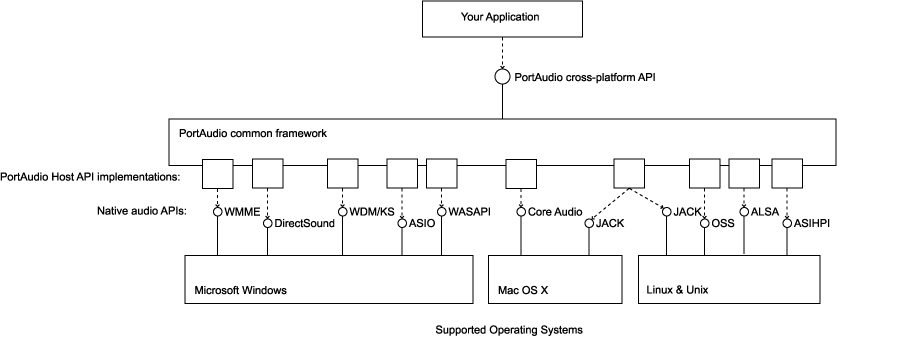
\includegraphics[scale=0.4,trim=0 0 0 0]{portaudio_architecture.png}%trim=l b r t
	\caption{This is an overview of the PortAudio interface.}
	\label{fig:app_portaudio}
	\end{center}
\end{figure}

\footnotetext{\url{http://www.portaudio.com/}}
\end{description}%not sure if this should be here at all, yet
%
\end{document}